\chapter{Testing della scheda}

Testando con l’oscilloscopio un segnale di prova di pilotaggio dei motori ci 
siamo accorti che in uscita non si aveva il segnale desiderato. 
Perciò prima abbiamo testato il segnale PWM generato dal microcontrollore, 
il quale è risultato corretto.\\
Poi siamo passati al test sul MOSFET di pilotaggio.\\
Qui ci siamo accorti che il segnale era sbagliato, quindi abbiamo intuito che il problema fossero i transistor.
Il professore ci ha poi aiutati a capire nel dettaglio il problema misurando la tensione ai capi del diodo di
protezione tra drain e source del MOSFET. Risultando un cortocircuito tra drain e source abbiamo capito che 
quelli non erano realmente il drain e il source del MOSFET e che quindi il transistor era stato saldato in 
modo errato. Effettuando la misurazione di tensione tra i vari pin del transistor abbiamo capito quale fosse il gate.
Successivamente abbiamo girato i transistor come descritto nell’assemblaggio e, dopo altri test, il sistema di pilotaggio
degli stepper è risultato funzionante.\\

Il consumo del prototipo è stato misurato all’avviamento dei motori e in modalità idle, dai quali abbiamo ricavato le seguenti misure:
\begin{itemize}
\item
    \begin{quote}
    consumo istantaneo a 1/1.5 W
    \end{quote}
\item
    \begin{quote}
    consumo in idle 0.2/0.4 W
    \end{quote}
\end{itemize}


\begin{center}
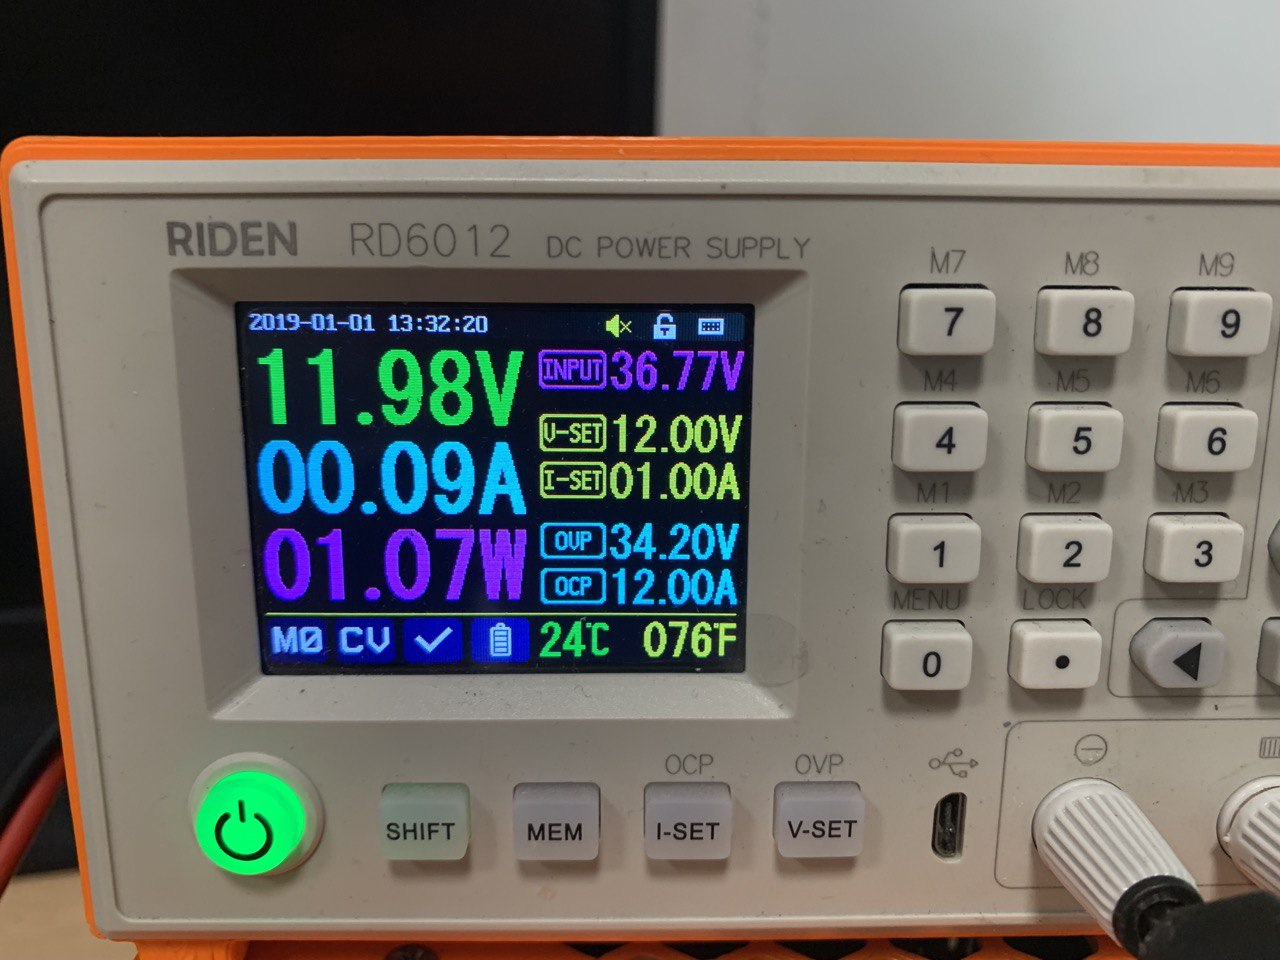
\includegraphics[scale=0.3]{figures/image3.png}
\captionsetup{type=figure}
\captionof{figure}{Consumi durante il movimento dei motori}
\end{center}

\begin{center}
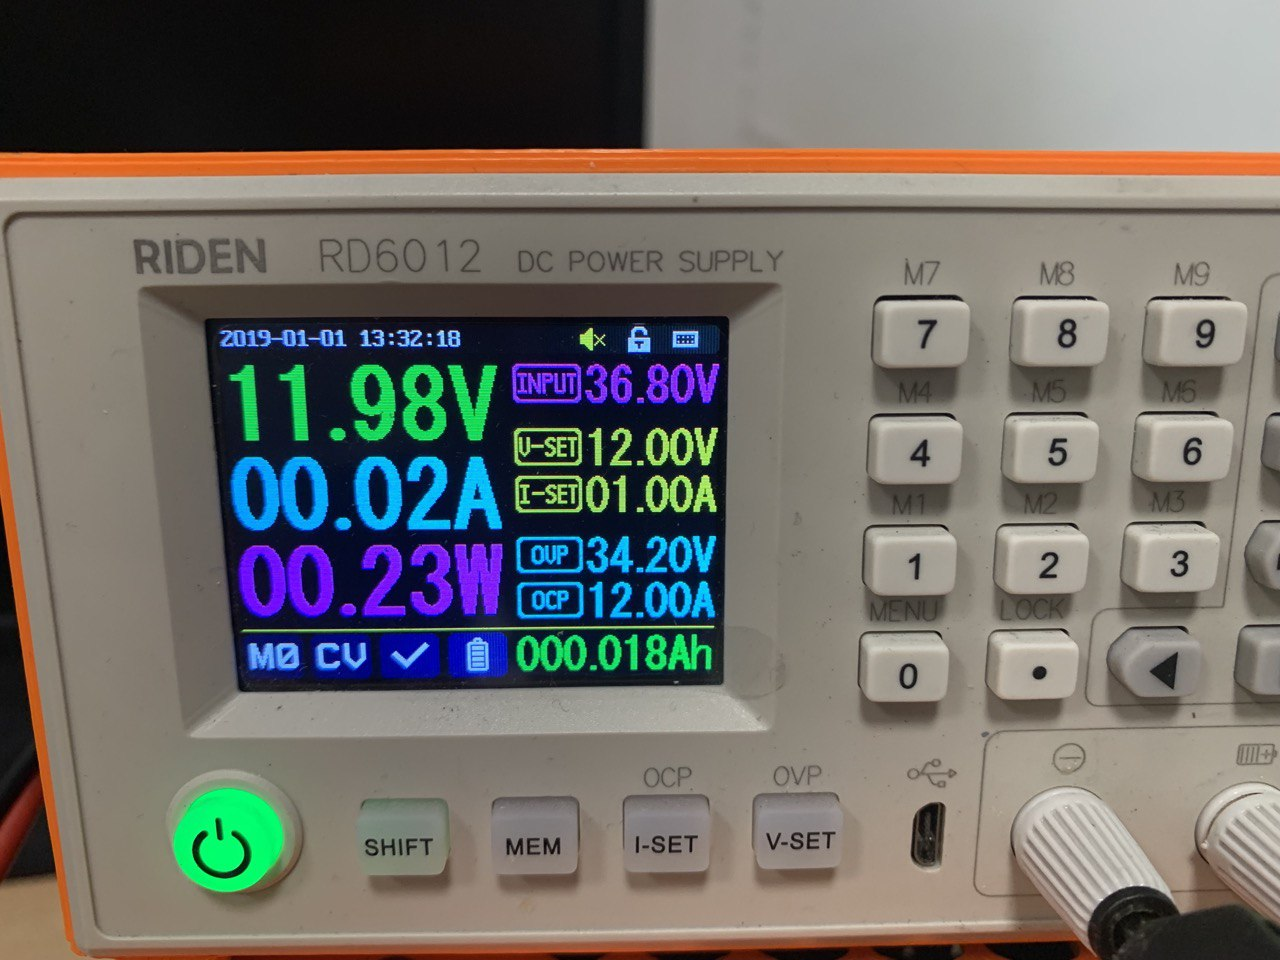
\includegraphics[scale=0.3]{figures/image1.png}
\captionsetup{type=figure}
\captionof{figure}{Consumi durante lo stato di idle}
\end{center}

I consumi dei motori sono complessivamente bassi poiché, grazie alla loro coppia statica elevata, non è necessario
alimentarli per far sì che mantengano la posizione.
